\documentclass[12pt, a4paper]{article}
\usepackage{graphicx}
\usepackage{amsmath}
\usepackage{hyperref}


\begin{document}
\title{Sea-ice Flow Simplified}
\author{Kecheng Zhang}
\maketitle


\section{Introduction}
Se-ice flow is the study of the movement of sea ice. It is an important topic in the study of climate change. The movement of sea ice is affected by many factors, such as wind, ocean currents, and temperature.
This project aims to model the movement of sea ice using a feed forward neural network. The model is trained using the data of the speed of the piece of sea ice at different positions. The model is then used to predict the movement of the sea ice over a period of time.
This paper will first introduce the mathematics behind the model, then the neural network structure, and finally the performance of the model.
\section{Method}

\subsection{Mathematics}
The ocean velocity field can be modeled as
$$ U = 0.5 + 0.3sin(2 \pi x) $$
where x is the position of the piece, and we have data
$x_1(0) = 0.3$, $x_2(0) = 0.7$, and $v_1(0) = v_2(0) = 0$.
We want to calculate
$x_k(t_j)$ and $v_k(t_j)$ for $k = 1, 2$ and $j = 1\dots10000$, where
$\delta t = 10^{-3}$ and $t_j = \delta t j$, such that
$$\begin{cases}
    \frac{\partial x_k}{\partial t} = v_k\\
    \frac{\partial v_k}{\partial t} = (u - v_k) |u - v_k|\\
    \end{cases}$$
and $$ \frac{x_k(t_{j+1}) - x_k(t_j)}{dt} = v_k(t_j)$$

\subsection{Neural Network}
The neural network is a feed-forward network with 2 hidden layers shown in Figure 1. The loss funciton used to train the model is the sum of two loss functions, the displacement and the momentum, which are defined as
$$Loss = \Sigma^2_{k=1}(x_k - x_{k,in} - v_k\delta t)^2 + \Sigma^2_{k=1}(v_k - v_{k,in} - (u - v_k) |u - v_k|\delta t)^2$$

\begin{figure}
    \centering
    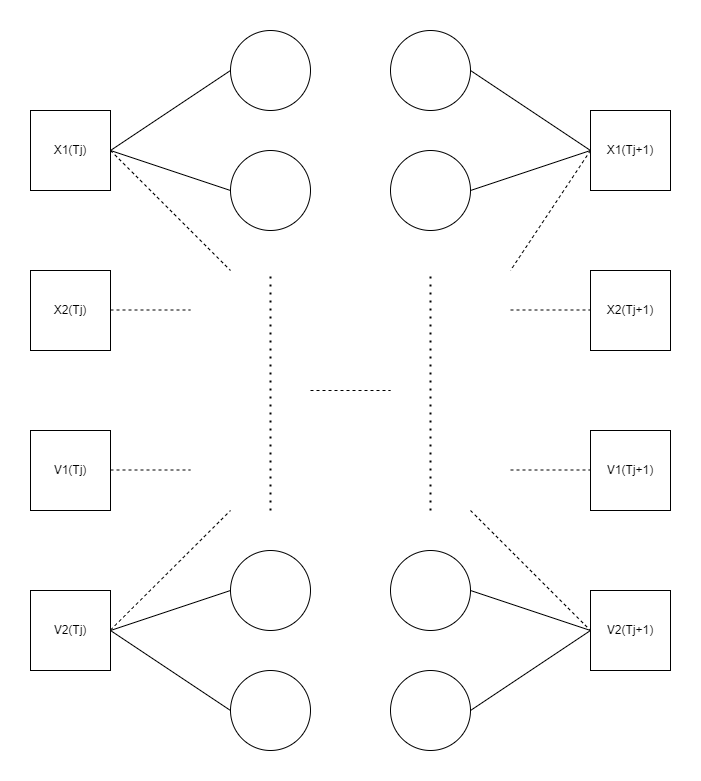
\includegraphics[scale=0.3]{../NN_graph.png}
    \caption[]{Neural Network structure}
    \label{fig:neural_network}
\end{figure}

\section{Discussion}
\subsection{Performance}
The performance of the feed forward neural network was evaluated based on its ability to replicate the physical behavior of sea-ice flow over a specified time frame, which has shown both significance and challenges. 

The model requires little computational resources, and is capable to model the sea-ice flow with good accuracy in short amount of time. However, the error accumulates which leads to a reduction in accuracy as time increases.

Figure 2 shows the training loss and tesing loss respectivly. The tesing error has shown a increasing trend due to the accumulation of the error in each time step. The training loss decreases as time increases, which suggests the model converges.

\begin{figure}
    \centering
    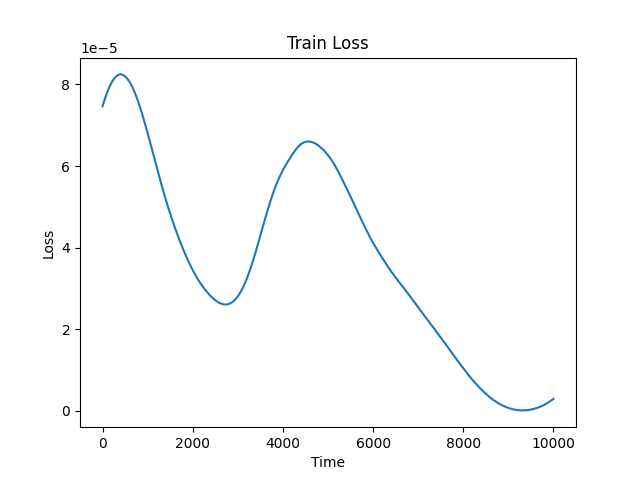
\includegraphics[scale=0.4]{../Train_loss.png}
    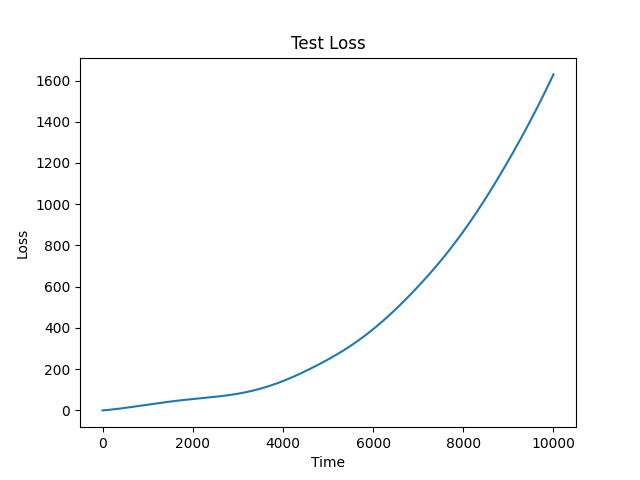
\includegraphics[scale=0.4]{../Test_loss.png}
    \caption[]{Training and testing loss}
    \label{fig:loss}
\end{figure}

\subsection{Weighted Loss}
In addition to the loss function defined in the mathematics section, a weighted loss function is also tested. The weighted loss function is defined as
$$ Loss_{weighted} = Loss \times j$$
where $j$ is the time step. The weighted loss function is expected to reduce the error accumulation since the error is penatized more as time increases. Figure 3 shows the training loss and testing loss of the model using weighted loss function. 

\begin{figure}
    \centering
    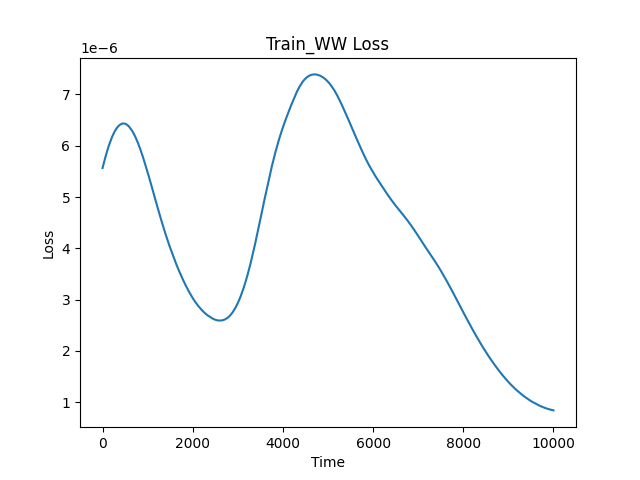
\includegraphics[scale=0.4]{../Train_WW_loss.png}
    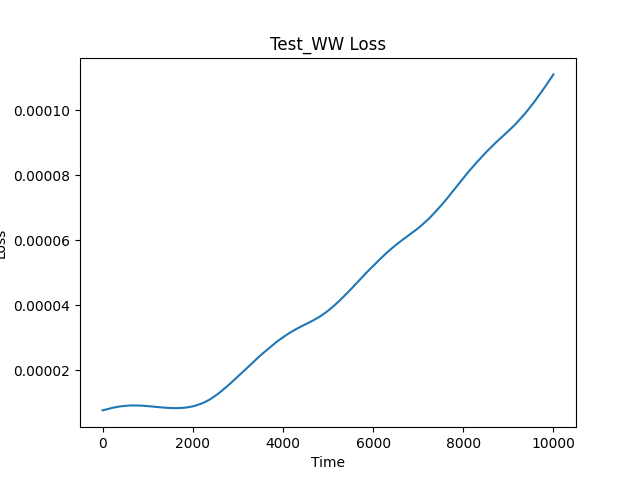
\includegraphics[scale=0.4]{../Test_WW_loss.png}
    \caption[]{Training and testing loss using weighted loss function}
    \label{fig:loss_ww}
\end{figure}

Using weighted loss function has shown a better performance in terms of reducing the error accumulation. Figure 5 shows the mean square error of the model of the two methods. Figure 4 shows the model using weighted loss function has a lower mean square error (0.00011) compair to the one without weighted loss function (0.00155).

\begin{figure}
    \centering
    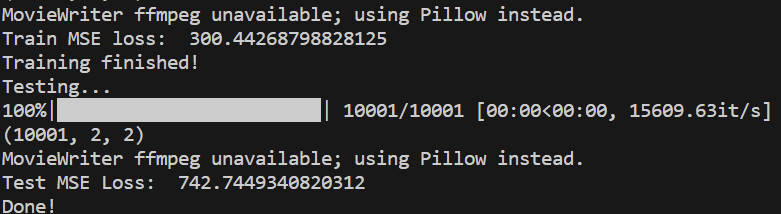
\includegraphics[scale=0.7]{../mse.png}
    \caption[]{Training and testing loss}
    \label{fig:mse1}
\end{figure}

\subsection*{Different Ocean Velocity Field}
An alternative ocean velocity field with different initial state is used to test the performance. The field is defined as:
$$ U = 0.2 + 0.5sin(2 \pi x) $$

\begin{figure}
    \centering
    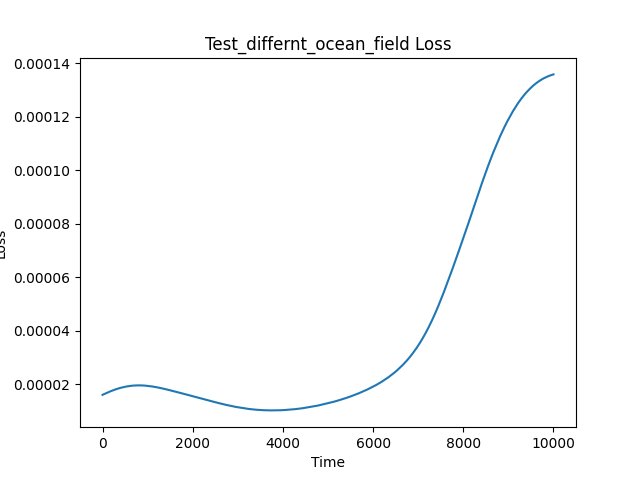
\includegraphics[scale=0.7]{../Test_differnt_ocean_field_loss.png}
    \caption[]{Testing loss using different ocean velocity field}
    \label{fig:loss_different_ovf}
\end{figure}

Figure 5 shows the testing loss of the model using different ocean velocity field. The mean suqre error retrieved was 0.00014, while using same velocity field is 0.00024 (Figure 6).

\begin{figure}
    \centering
    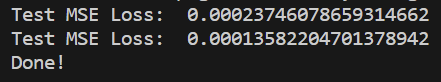
\includegraphics[scale=1]{../mse2.png}
    \caption[]{Testing loss of origional field and different field}
    \label{fig:mse2}
\end{figure}

\section{Conclusion}
In conclusion, the feed forward neural network is capable to model the sea-ice flow with good accuracy, and robust enough to predict the movement of ice with different ocean velocity field. In addition, the use of weighted loss function has proven to be effective in reducing the error accumulation.

\newpage
\section{Appendix}
Code: 
\href{https://github.com/Kecheng-Zhang/Sea-ice-flow-simplified}{https://github.com/Kecheng-Zhang/Sea-ice-flow-simplified}

\end{document}